\documentclass[main.tex]{subfiles}

\begin{document}
\subsection{Overall Concurrency Control Architecture}

\begin{figure}[!hbt]
	\centering
	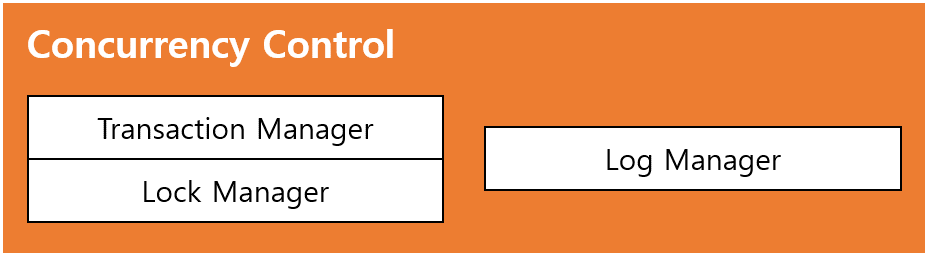
\includegraphics[width=.7\textwidth]{images/cc/overall_design.png}
	\caption{Overall Design of Concurrency Control}
	\label{cc:overall_design}
\end{figure}

Figure \ref{cc:overall_design}는 \texttt{Concurrency Control}의 전반적인 구조도다. \texttt{Concurrency Control}은 크게 transaction과 lock을 관리하는 부분과 logging을 관리하는 부분으로 나뉜다.

\subsubsection{Transaction Manager}
\begin{table}[!htb]
	\begin{tabularx}{\textwidth}{|l|X|}
		\hline
		\textbf{File} & xact.h xact.cpp \\
		\hline
		\textbf{Class} & XactManager Xact \\
		\hline
		\textbf{Purpose} & Transaction의 발급, commit, abort 등을 담당한다. \\
		\hline
	\end{tabularx}
\end{table}

\subsubsection{Lock Manager}
\begin{table}[!htb]
	\begin{tabularx}{\textwidth}{|l|X|}
		\hline
		\textbf{File} & lock.h lock.cpp \\
		\hline
		\textbf{Class} & LockManager Lock HashTableEntry WFGNode \\
		\hline
		\textbf{Purpose} & 각 record에 대한 lock을 관리한다. \\
		\hline
	\end{tabularx}
\end{table}

\subsubsection{Log Manager}
\begin{table}[!htb]
	\begin{tabularx}{\textwidth}{|l|X|}
		\hline
		\textbf{File} & log.h log.cpp \\
		\hline
		\textbf{Class} & LogManager Log \\
		\hline
		\textbf{Purpose} & Log를 발급하고 log를 stable storage에 저장하고 불러오는 역할을 담당한다. \\
		\hline
	\end{tabularx}
\end{table}

\subsection{Transaction Processing}

\subsubsection{Lock Management}
\paragraph{Lock}
Lock엔 SHARED mode와 EXCLUSIVE mode가 존재한다.
SHARED mode에서는 다른 transaction과 동시에 한 record에 대한 lock을 가질 수 있지만,
EXCLUSIVE mode의 lock을 어느 한 transaction이 획득하면 commit 혹은 abort가 되기 전까지 다른 transaction에서 해당 record에 대한 lock을 획득하지 못해 wait 해야 한다.

\begin{figure}[!hbt]
	\centering
	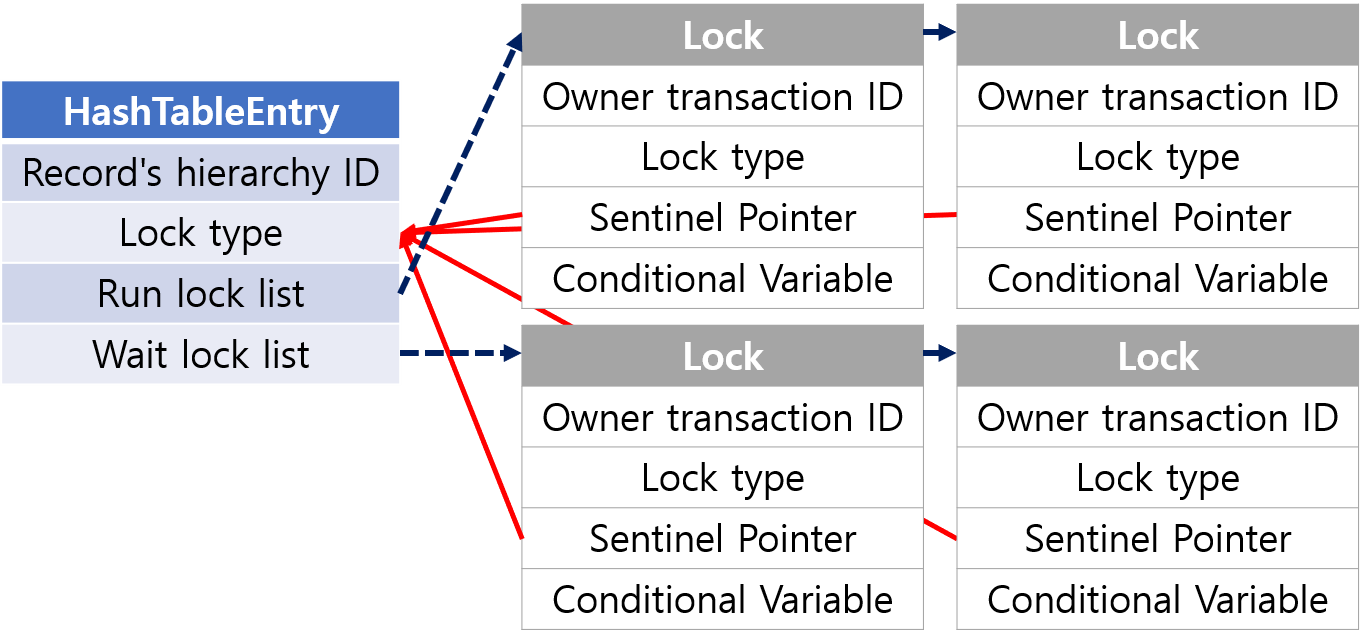
\includegraphics[width=.7\textwidth]{images/cc/lock_structure.png}
	\caption{Overall Lock Architecture}
\end{figure}

HashTableEntry의 Lock type은 해당 record에 걸린 lock 중 가장 강력한 lock type을 나타낸다.
예컨대 SHARED mode의 lock과 EXCLUSIVE mode의 lock이 동시에 한 record에 걸려있다면 해당 record에 대한 HashTableEntry의 Lock type은 EXCLUSIVE가 된다
(단, 아무 lock이 존재하지 않는다면 None이다).

그리고 lock acquire가 성공한 lock object의 list와 성공하지 못해 wait 상태인 lock의 object의 list를 별도로 두었다.
이렇게 디자인한 사유는 구현의 편의와 효율성을 위해서다.
lock acquire에서 acquire 혹은 wait 여부를 결정할 때 하나의 list로 관리한다면 깨어있는 lock과 대기 중인 lock의 경계를 찾기 위해 list를 순회하는데 $O(n)$의 time complexity가 발생한다.
하지만 둘을 분리함으로써 run lock list의 마지막과만 비교하는 $O(1)$의 time complexity로 해결이 가능하다.

\paragraph{Hash Table}
(table id, page id, offset)에 해당하는 HashTableEntry를 빠르게 찾기 위해 searching structure로 hash table을 두었다. Hash table의 구현체는 STL library의 unordered\_map을 이용하였다.
hashing function은 STL library에 있는 문자열에 대한 hashing function을 이용하여 만들었다.

\begin{algorithm}
	\caption{Hash function for tuple of (table id, page id, offset)}
	
	\begin{algorithmic}[lines]
		\Function{Hash}{table id, page id, offset}
		\State \Return {StringHashing(table id + "$|$" + page id +\\
			\hspace{0.3\linewidth} "$|$" + offset)}
		\Comment{StringHashing은 STL library}
		\EndFunction
	\end{algorithmic}
\end{algorithm}

\newpage
\paragraph{Optimization for Condition Variable}
Lock object 별로 condition variable을 가지고 있는 디자인(non-shared)과 HashTableEntry에서 만 condition variable을 갖도록 하는 디자인(shared)을 각각 구현해 성능 테스트를 하여 다음과 같이 전자의 디자인의 성능이 더 우수함을 확인했다.

\begin{figure}[!hbt]
	\centering
	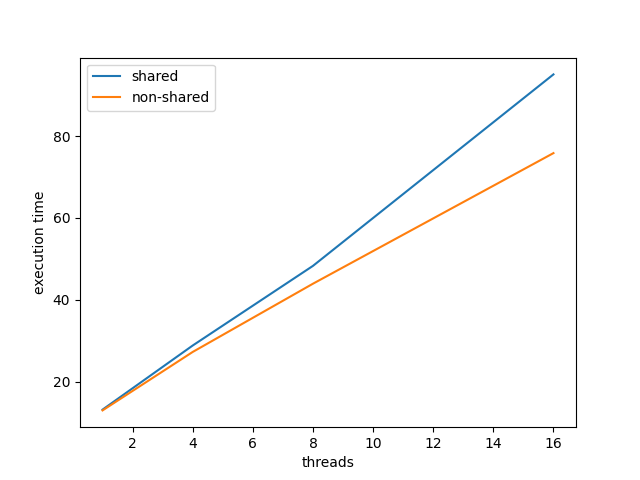
\includegraphics[width=.8\textwidth]{images/cc/cond_var_design.png}
	\caption{Performance Test for Condition Variable Design}
\end{figure}



\paragraph{Lock Acquire}\mbox{}\\
Lock을 acquire할 수 있다면 HashTableEntry의 run lock list에 넣는다. Lock의 획득 조건은 다음과 같다.\mbox{}\\

\noindent \textbf{(1) 현재 깨어있는 lock이 존재하지 않을 때}\\
\indent 이 경우는 해당 record를 사용하고 있는 transaction이 없다는 의미이므로 lock을 바로 획득할 수 있다.
\mbox{}\\

\noindent \textbf{(2) 대기 중인 lock이 없으며 entry의 lock type이 SHARED이고 lock의 type도 SHARED일 때}\\
\indent 이 경우엔 해당 record를 변경한 transaction이 존재하지 않은 경우이며, 또한 해당 lock을 통해서 하는 작업도 해당 record를 수정하지 않기에 dirty read, inconsistent read 등이 발생하지 않는다. 따라서 이 경우에도 lock을 바로 획득할 수 있다.
\mbox{}\\

\noindent \textbf{(3) 대기 중인 lock이 없으며 실행 중인 마지막 lock과 현재 요청하는 lock이 같은 transaction에 속할 때}\\
\indent 같은 transaction에서 수행되는 작업은 lock으로 보호될 필요가 없다. 따라서 이 경우에도 lock을 바로 획득할 수 있다.
\mbox{}\\

\noindent \textbf{(4) lock type이 SHARED이며 대기 중인 lock이 존재하지만 전부 SHARED인 경우}\\
\begin{figure}[!hbt]
	\centering
	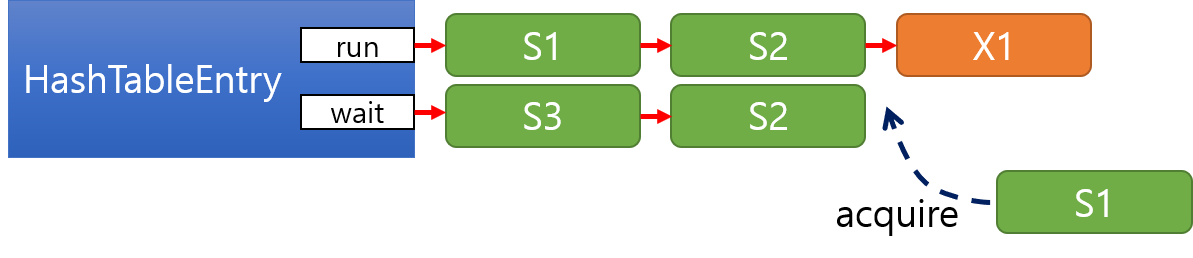
\includegraphics[width=.8\textwidth]{images/cc/lock_acquire_4.png}
\end{figure}

\indent 위 그림과 같은 상황이다. 이때 S1은 wait에서 대기 중인 S3와 S2와 conflict가 나지 않는다. 따라서 S1은 제일 앞으로 순서를 바꾸어 생각해도 무방하며, 그 결과 실질적으로 위 3번과 같은 상황이 된다면 lock을 바로 획득할 수 있다.

\paragraph{Lock Wait}
Lock을 acquire 하는데 실패했다면 해당 lock이 deadlock을 유발하는지를 검사한다. 만약 deadlock을 유발하지 않는다면 HashTableEntry의 wait lock list에 넣고 대기한다.


\paragraph{Lock Release}\mbox{}\\
우선 release 할 lock을 lock list에서 지운다. 그 후 남은 lock을 다음 절차에 따라 관리한다.\mbox{}\\

\noindent \textbf{(1) run lock list가 비어있지 않은 경우}\\
\indent wait에 있는 lock은 현재 run에 속한 lock과 충돌 나는 것들이다. 따라서 깨울 수 있는 wait에 속한 lock은 존재하지 않아 추가 작업 없이 바로 종료한다.
\mbox{}\\

\noindent \textbf{(2) wait lock list가 비어있는 경우}\\
\indent run과 wait 모두 비어있는 경우엔 더는 해당 record에 대한 lock이 없다는 의미이므로 lock hash table에서 해당 entry를 지우고 종료한다.
\mbox{}\\

\noindent \textbf{(3) wait lock list의 가장 선행하는 lock이 EXCLUSIVE일 경우}\\
\indent entry의 lock type을 EXCLUSIVE로 두고, 해당 lock만 깨우고 종료한다. 제일 처음에 있는 lock이 EXCLUSIVE일 때 그 이후에 있는 lock은 conflict 관계에 있기 때문에 오직 제일 앞의 lock만 깨우면 된다.
\mbox{}\\

\noindent \textbf{(4) wait lock list의 가장 선행하는 lock이 SHARED일 경우}\\
\indent entry의 lock type을 SHARED로 두고, 이후에 다시 EXCLUSIVE lock이 있기 직전까지의 모든 lock을 깨운다.
\mbox{}\\

\subsubsection{Deadlock Detection}

\paragraph{Wait for Graph}
Deadlock은 \emph{Wait for Graph}를 만들어 cycle이 존재하는지 확인하는 방식으로 탐지한다.

\newpage
\begin{figure}[!hbp]
	\centering
	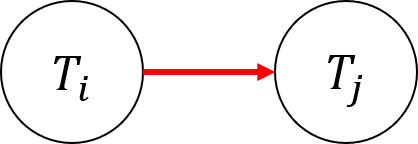
\includegraphics[width=.4\textwidth]{images/cc/wait_for_graph.png}
	
	$T_i$ : running transaction, $T_j$ : wait for $T_i$
	
	\caption{Wait for Graph}
\end{figure}

\noindent 만약 Wait for Graph상에 cycle이 존재하는 경우는 각 transaction이 서로를 기다리는 상황이다. 따라서 이 경우 deadlock이 발생한 것으로 판단할 수 있다.

\paragraph{Deadlock Detection Process}\mbox{}\\
Deadlock 탐지는 다음 순서에 따라 진행된다.\mbox{}\\

\noindent \textbf{(1) Build Wait for Graph}\\
\indent \texttt{Lock Manager}에 등록된 모든 lock에 대하여 wait-for-graph를 만든다. 각 node는 선행되어 실행된 node의 xact ID의 set인 In과 이후에 선행된 lock을 기다리는 node의 xact ID의 set인 Out. 그리고 DFS를 위한 변수 exploring과 visited로 이루어진다.
\mbox{}\\

\noindent \textbf{(2) Check Cycle}\\
\indent deadlock check이 실행되는 시점은 어떤 lock이 wait 되기 직전이므로 해당 lock에 관련된 node만 탐색해주면 된다. 따라서 해당 lock의 transaction에 대응되는 node를 시작점으로 하여 Depth First Search (DFS)를 통해 cycle을 탐색한다.
\mbox{}\\

\noindent \textbf{(3) Abort and Rollback}\\
\indent 위 process 진행 결과 cycle이 존재한다 판별되면 요청 들어온 lock에 대응하는 transaction을 abort 및 rollback 한다.
\mbox{}\\

\subsubsection{Transaction}
\begin{figure}[!hbt]
	\centering
	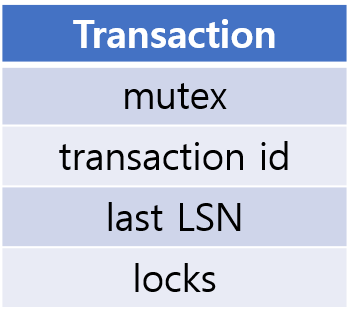
\includegraphics[width=.3\textwidth]{images/cc/transaction.png}
	\caption{Transaction Structure}
\end{figure}

\paragraph{Lock}
Transaction은 \texttt{Index Management Layer}와 \texttt{Lock Manager} 사이에 연결을 담당한다.
\texttt{Index Management Layer}에서 특정 record에 접근할 때는 transaction에 필요한 lock을 요청하며,
해당 transaction이 \texttt{Lock Manager}에게 해당 lock을 요청한다. 그 뒤 획득한 lock을 lock list에 저장한다.

\begin{figure}[!hbt]
	\centering
	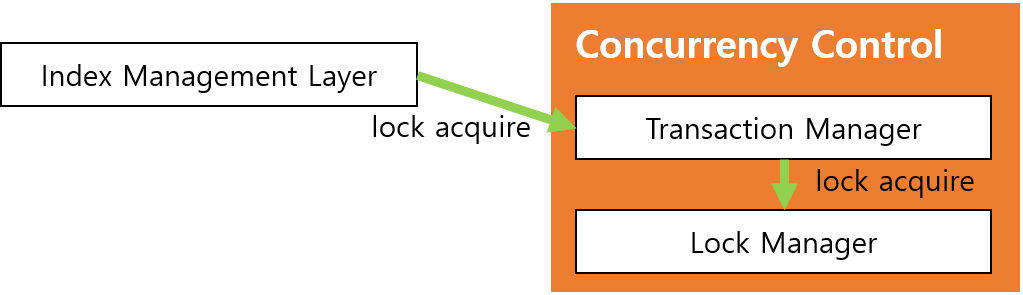
\includegraphics[width=.8\textwidth]{images/cc/lock_acquire.png}
	\caption{How to acquire lock in \texttt{Index Management Layer}}
\end{figure}

\paragraph{Commit}
Transaction이 정상적으로 수행된 뒤 commit 명령이 들어오면 다음의 순서대로 작업을 수행한다.

\begin{enumerate}
	\item 해당 transaction이 획득한 모든 lock을 release
	\item \texttt{Log Manager}에 commit log 남기기
	\item \texttt{Transaction Manager}에서 해당 transaction 제거
\end{enumerate}

\paragraph{Abort and Rollback}
Transaction을 abort 하는 경우 해당 transaction이 database에 수정한 작업이 있다면 해당 부분을 전부 원래대로 돌려야 한다.
따라서 commit에 비해 rollback 작업이 추가로 필요하며, abort는 다음의 순서대로 작업을 수행한다.

\begin{enumerate}
	\item 해당 transaction이 수행한 모든 작업을 rollback
	\item 해당 transaction이 획득한 모든 lock을 release
	\item \texttt{Log Manager}에 rollback log 남기기
	\item \texttt{Transaction Manager}에서 해당 transaction 제거
\end{enumerate}

\begin{figure}[!hbt]
	\centering
	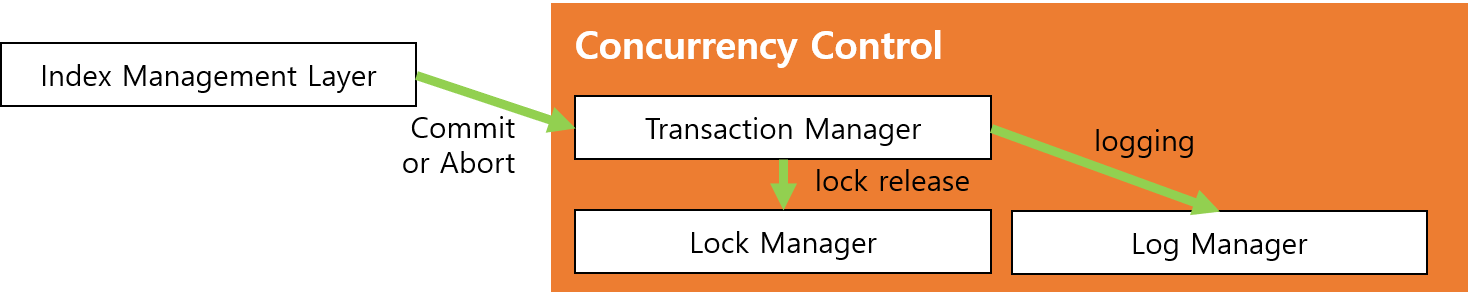
\includegraphics[width=.9\textwidth]{images/cc/commit_abort.png}
	\caption{Commit or Abort}
\end{figure}

\end{document}
